\documentclass[8pt,aspectratio=169]{beamer}
\usetheme{Madrid}
\usepackage{graphicx,booktabs,adjustbox,multicol,amsmath,amssymb,listings,xcolor}
\definecolor{mlblue}{RGB}{0,102,204}
\definecolor{mlpurple}{RGB}{51,51,178}
\definecolor{mllavender}{RGB}{173,173,224}
\definecolor{mllavender2}{RGB}{193,193,232}
\definecolor{mllavender3}{RGB}{204,204,235}
\definecolor{mllavender4}{RGB}{214,214,239}
\definecolor{mlorange}{RGB}{255,127,14}
\definecolor{mlgreen}{RGB}{44,160,44}
\definecolor{mlred}{RGB}{214,39,40}
\definecolor{mlgray}{RGB}{127,127,127}
\definecolor{solkeyword}{RGB}{0,102,153}
\setbeamercolor{palette primary}{bg=mllavender3,fg=mlpurple}
\setbeamercolor{palette secondary}{bg=mllavender2,fg=mlpurple}
\setbeamercolor{palette tertiary}{bg=mllavender,fg=white}
\setbeamercolor{palette quaternary}{bg=mlpurple,fg=white}
\setbeamercolor{structure}{fg=mlpurple}
\setbeamercolor{title}{fg=mlpurple}
\setbeamercolor{frametitle}{fg=mlpurple,bg=mllavender3}
\setbeamercolor{block title}{bg=mllavender2,fg=mlpurple}
\setbeamercolor{block body}{bg=mllavender4,fg=black}
\setbeamertemplate{navigation symbols}{}
\setbeamertemplate{itemize items}[circle]
\setbeamersize{text margin left=5mm,text margin right=5mm}
\newcommand{\bottomnote}[1]{\vfill\vspace{-2mm}\textcolor{mllavender2}{\rule{\textwidth}{0.4pt}}\vspace{1mm}\footnotesize\textbf{#1}}
\usepackage{tikz,pgfplots}
\pgfplotsset{compat=1.18}
\usetikzlibrary{arrows.meta,positioning,shapes.geometric,calc}
\title{NFTs \& Digital Assets: Course Preview}
\subtitle{INTRO Preview}
\author{Prof.~Dr.~Joerg Osterrieder}
\institute{University Lecture Series}
\date{\today}
\begin{document}

% Frame 1: Title
\begin{frame}
\titlepage
\end{frame}

% Frame 2: Why NFTs Matter
\begin{frame}{Why NFTs Matter}
\begin{columns}[T]
\begin{column}{0.62\textwidth}
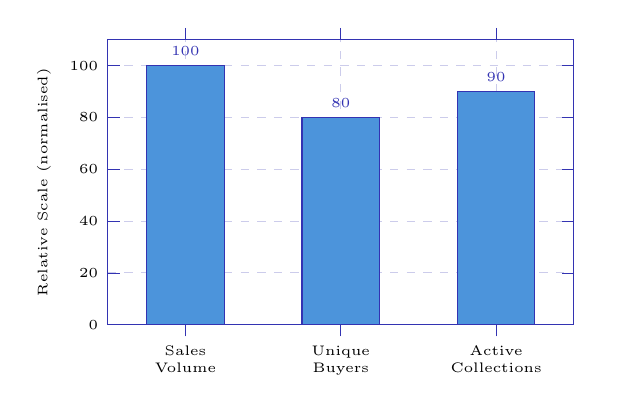
\begin{tikzpicture}
\begin{axis}[
  ybar,
  bar width=28pt,
  width=7.5cm,
  height=5.2cm,
  symbolic x coords={Sales Volume, Unique Buyers, Collections},
  xtick=data,
  xticklabels={Sales\\Volume, Unique\\Buyers, Active\\Collections},
  xticklabel style={font=\tiny, text width=2.5cm, align=center},
  ymin=0, ymax=110,
  ytick={0,20,40,60,80,100},
  yticklabel style={font=\tiny},
  ylabel style={font=\tiny},
  ylabel={Relative Scale (normalised)},
  axis line style={draw=mlpurple},
  tick style={draw=mlpurple},
  nodes near coords,
  nodes near coords style={font=\tiny, color=mlpurple},
  point meta=y,
  enlarge x limits=0.25,
  grid=major,
  grid style={dashed, mllavender3},
]
\addplot[fill=mlblue!70, draw=mlpurple] coordinates {
  (Sales Volume,  100)
  (Unique Buyers,  80)
  (Collections,    90)
};
\end{axis}
\end{tikzpicture}
\end{column}
\begin{column}{0.36\textwidth}
\vspace{4mm}
\begin{block}{Key Metrics}
\begin{itemize}\setlength\itemsep{4pt}
  \item[\small$\checkmark$] \small \textbf{\$25B+} peak annual sales
  \item[\small$\checkmark$] \small \textbf{2M+} unique buyers/sellers
  \item[\small$\checkmark$] \small \textbf{100K+} active collections
  \item[\small$\checkmark$] \small Gaming/art/real estate applications
\end{itemize}
\end{block}
\end{column}
\end{columns}
\bottomnote{NFTs are reshaping digital ownership across art, gaming, and real-world assets.}
\end{frame}

% Frame 3: NFT Ecosystem at a Glance
\begin{frame}{NFT Ecosystem at a Glance}
\vspace{2mm}
\begin{center}
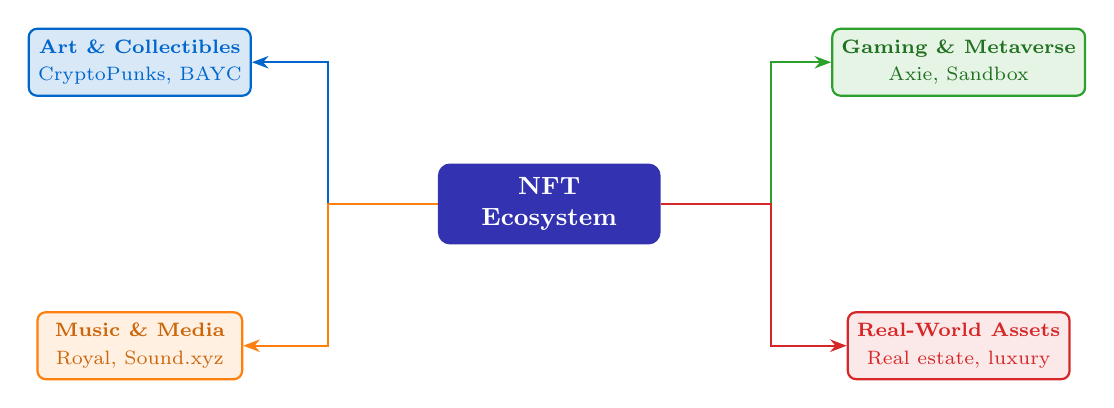
\begin{tikzpicture}[
  cbox/.style={rectangle, rounded corners=4pt, draw=mlpurple, thick,
               fill=mlpurple, minimum width=2.8cm, minimum height=1.0cm,
               font=\small\bfseries, align=center, text=white},
  sbox/.style={rectangle, rounded corners=3pt, thick,
               minimum width=2.6cm, minimum height=0.85cm,
               font=\scriptsize, align=center},
  arr/.style={-{Stealth[length=6pt]}, thick}
]
% Center node
\node[cbox] (center) at (0,0) {NFT\\Ecosystem};

% Spoke nodes
\node[sbox, draw=mlblue,   fill=mlblue!15,   text=mlblue]              (art)  at (-5.2, 1.8)
  {\textbf{Art \& Collectibles}\\[2pt]CryptoPunks, BAYC};

\node[sbox, draw=mlgreen,  fill=mlgreen!12,  text=mlgreen!70!black]    (game) at ( 5.2, 1.8)
  {\textbf{Gaming \& Metaverse}\\[2pt]Axie, Sandbox};

\node[sbox, draw=mlorange, fill=mlorange!12, text=mlorange!80!black]   (music) at (-5.2,-1.8)
  {\textbf{Music \& Media}\\[2pt]Royal, Sound.xyz};

\node[sbox, draw=mlred,    fill=mlred!10,    text=mlred]               (rwa) at ( 5.2,-1.8)
  {\textbf{Real-World Assets}\\[2pt]Real estate, luxury};

% Arrows
\draw[arr, draw=mlblue]   (center.west) -- ++(-1.4,0) |- (art.east);
\draw[arr, draw=mlgreen]  (center.east) -- ++(1.4,0)  |- (game.west);
\draw[arr, draw=mlorange] (center.west) -- ++(-1.4,0) |- (music.east);
\draw[arr, draw=mlred]    (center.east) -- ++(1.4,0)  |- (rwa.west);
\end{tikzpicture}
\end{center}
\bottomnote{The NFT ecosystem spans digital and physical assets, with new use cases emerging rapidly.}
\end{frame}

% Frame 4: NFT Market Trajectory
\begin{frame}{NFT Market Trajectory}
\begin{columns}[T]
\begin{column}{0.62\textwidth}
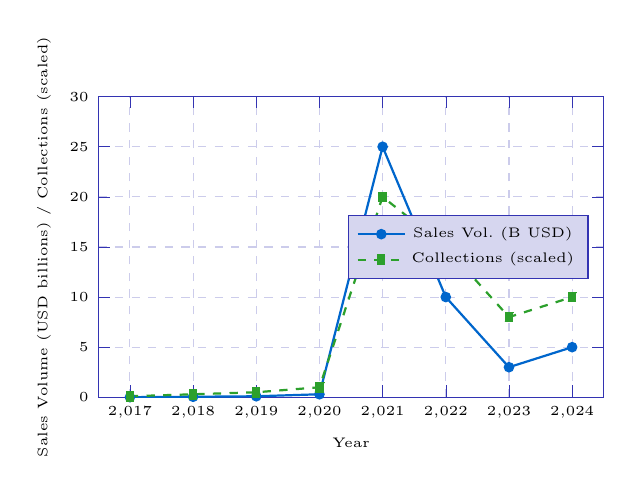
\begin{tikzpicture}
\begin{axis}[
  width=8.0cm,
  height=5.4cm,
  xmin=2016.5, xmax=2024.5,
  ymin=0, ymax=30,
  xtick={2017,2018,2019,2020,2021,2022,2023,2024},
  ytick={0,5,10,15,20,25,30},
  xticklabel style={font=\tiny},
  yticklabel style={font=\tiny},
  xlabel style={font=\tiny},
  ylabel style={font=\tiny},
  xlabel={Year},
  ylabel={Sales Volume (USD billions) / Collections (scaled)},
  axis line style={draw=mlpurple},
  tick style={draw=mlpurple},
  grid=major,
  grid style={dashed, mllavender3},
  legend style={font=\tiny, at={(0.97,0.5)}, anchor=east,
                fill=mllavender4, draw=mlpurple},
]
% Sales Volume line
\addplot[color=mlblue, solid, thick, mark=*, mark size=1.5pt] coordinates {
  (2017,0.01)(2018,0.05)(2019,0.1)(2020,0.3)(2021,25)(2022,10)(2023,3)(2024,5)
};
% Collections count (scaled to same axis)
\addplot[color=mlgreen, dashed, thick, mark=square*, mark size=1.5pt] coordinates {
  (2017,0.1)(2018,0.3)(2019,0.5)(2020,1)(2021,20)(2022,15)(2023,8)(2024,10)
};
\legend{Sales Vol.\ (B USD), Collections (scaled)}
\end{axis}
\end{tikzpicture}
\end{column}
\begin{column}{0.36\textwidth}
\vspace{4mm}
\begin{block}{Growth Drivers}
\begin{itemize}\setlength\itemsep{4pt}
  \item[\small$\checkmark$] \small \textbf{PFP collections} drove 2021 boom
  \item[\small$\checkmark$] \small \textbf{Gaming NFTs} sustaining utility
  \item[\small$\checkmark$] \small \textbf{RWA tokenization} emerging
  \item[\small$\checkmark$] \small \textbf{Regulatory clarity} improving
\end{itemize}
\end{block}
\end{column}
\end{columns}
\bottomnote{NFT market survived the 2022 downturn and is finding sustainable use cases.}
\end{frame}

% Frame 5: Course Coverage
\begin{frame}{Course Coverage}
\vspace{2mm}
\begin{center}
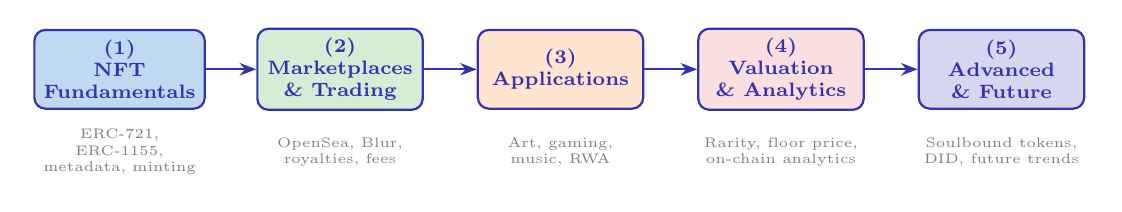
\begin{tikzpicture}[
  procstep/.style={
    rectangle, rounded corners=4pt,
    minimum width=2.1cm, minimum height=1.0cm,
    draw=mlpurple, thick,
    fill=mllavender3,
    font=\scriptsize\bfseries,
    align=center,
    text=mlpurple
  },
  conn/.style={-{Stealth[length=6pt]}, thick, draw=mlpurple}
]
\node[procstep, fill=mlblue!25]    (s1) at (0,0)    {(1)\\NFT\\Fundamentals};
\node[procstep, fill=mlgreen!20]   (s2) at (2.8,0)  {(2)\\Marketplaces\\\& Trading};
\node[procstep, fill=mlorange!20]  (s3) at (5.6,0)  {(3)\\Applications};
\node[procstep, fill=mlred!15]     (s4) at (8.4,0)  {(4)\\Valuation\\\& Analytics};
\node[procstep, fill=mlpurple!20]  (s5) at (11.2,0) {(5)\\Advanced\\\& Future};

\draw[conn] (s1) -- (s2);
\draw[conn] (s2) -- (s3);
\draw[conn] (s3) -- (s4);
\draw[conn] (s4) -- (s5);

\node[font=\tiny, text=mlgray, align=center, text width=2.1cm] at (0,-1.05)
  {ERC-721, ERC-1155,\\metadata, minting};
\node[font=\tiny, text=mlgray, align=center, text width=2.1cm] at (2.8,-1.05)
  {OpenSea, Blur,\\royalties, fees};
\node[font=\tiny, text=mlgray, align=center, text width=2.1cm] at (5.6,-1.05)
  {Art, gaming,\\music, RWA};
\node[font=\tiny, text=mlgray, align=center, text width=2.1cm] at (8.4,-1.05)
  {Rarity, floor price,\\on-chain analytics};
\node[font=\tiny, text=mlgray, align=center, text width=2.1cm] at (11.2,-1.05)
  {Soulbound tokens,\\DID, future trends};
\end{tikzpicture}
\end{center}
\vspace{4mm}
\begin{columns}[T]
\begin{column}{0.48\textwidth}
\begin{block}{Prerequisites}
\begin{itemize}\setlength\itemsep{2pt}
  \item[\small$\checkmark$] \small Basic blockchain and Ethereum knowledge
  \item[\small$\checkmark$] \small Familiarity with ERC-20 token standards
\end{itemize}
\end{block}
\end{column}
\begin{column}{0.48\textwidth}
\begin{block}{Outcomes}
\begin{itemize}\setlength\itemsep{2pt}
  \item[\small$\checkmark$] \small Evaluate NFT projects quantitatively
  \item[\small$\checkmark$] \small Analyse rarity, valuation, and market dynamics
\end{itemize}
\end{block}
\end{column}
\end{columns}
\bottomnote{From NFT fundamentals to advanced topics in 55 frames.}
\end{frame}

% Frame 6: What You Will Learn
\begin{frame}{What You Will Learn}
\begin{columns}[T]
\begin{column}{0.44\textwidth}
\vspace{2mm}
\begin{block}{Learning Outcomes}
\begin{itemize}\setlength\itemsep{5pt}
  \item[\small$\checkmark$] \small \textbf{NFT standards} --- ERC-721, ERC-1155, metadata schemas
  \item[\small$\checkmark$] \small \textbf{Marketplace analysis} --- fees, royalties, and liquidity dynamics
  \item[\small$\checkmark$] \small \textbf{Valuation metrics} --- rarity scoring and floor price models
  \item[\small$\checkmark$] \small \textbf{Future directions} --- soulbound tokens and real-world asset tokenization
\end{itemize}
\end{block}
\end{column}
\begin{column}{0.54\textwidth}
\vspace{2mm}
\begin{center}
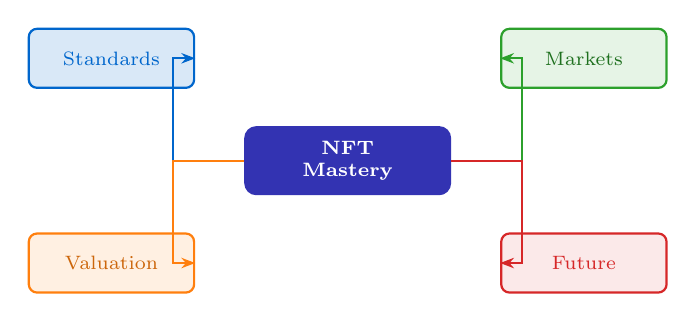
\begin{tikzpicture}[
  cbox/.style={rectangle, rounded corners=4pt, draw=mlpurple, thick,
               fill=mlpurple, minimum width=2.6cm, minimum height=0.85cm,
               font=\scriptsize\bfseries, align=center, text=white},
  fbox/.style={rectangle, rounded corners=3pt, thick,
               minimum width=2.1cm, minimum height=0.75cm,
               font=\scriptsize, align=center},
  farr/.style={-{Stealth[length=5pt]}, thick}
]
% Central node
\node[cbox] (nm) at (0,0) {NFT\\Mastery};

% Skill nodes
\node[fbox, draw=mlblue,   fill=mlblue!15,   text=mlblue]              (std)  at (-3.0, 1.3) {Standards};
\node[fbox, draw=mlgreen,  fill=mlgreen!12,  text=mlgreen!70!black]    (mkt)  at ( 3.0, 1.3) {Markets};
\node[fbox, draw=mlorange, fill=mlorange!12, text=mlorange!80!black]   (val)  at (-3.0,-1.3) {Valuation};
\node[fbox, draw=mlred,    fill=mlred!10,    text=mlred]               (fut)  at ( 3.0,-1.3) {Future};

% Arrows
\draw[farr, draw=mlblue]   (nm.west)  -- ++(-0.9,0) |- (std.east);
\draw[farr, draw=mlgreen]  (nm.east)  -- ++(0.9,0)  |- (mkt.west);
\draw[farr, draw=mlorange] (nm.west)  -- ++(-0.9,0) |- (val.east);
\draw[farr, draw=mlred]    (nm.east)  -- ++(0.9,0)  |- (fut.west);
\end{tikzpicture}
\end{center}
\end{column}
\end{columns}
\vspace{1mm}
\bottomnote{By the end you will be able to evaluate any NFT project quantitatively.}
\end{frame}

\end{document}
